\documentclass{standalone}
\usepackage{tikz}
\usetikzlibrary{patterns, positioning}

\begin{document}
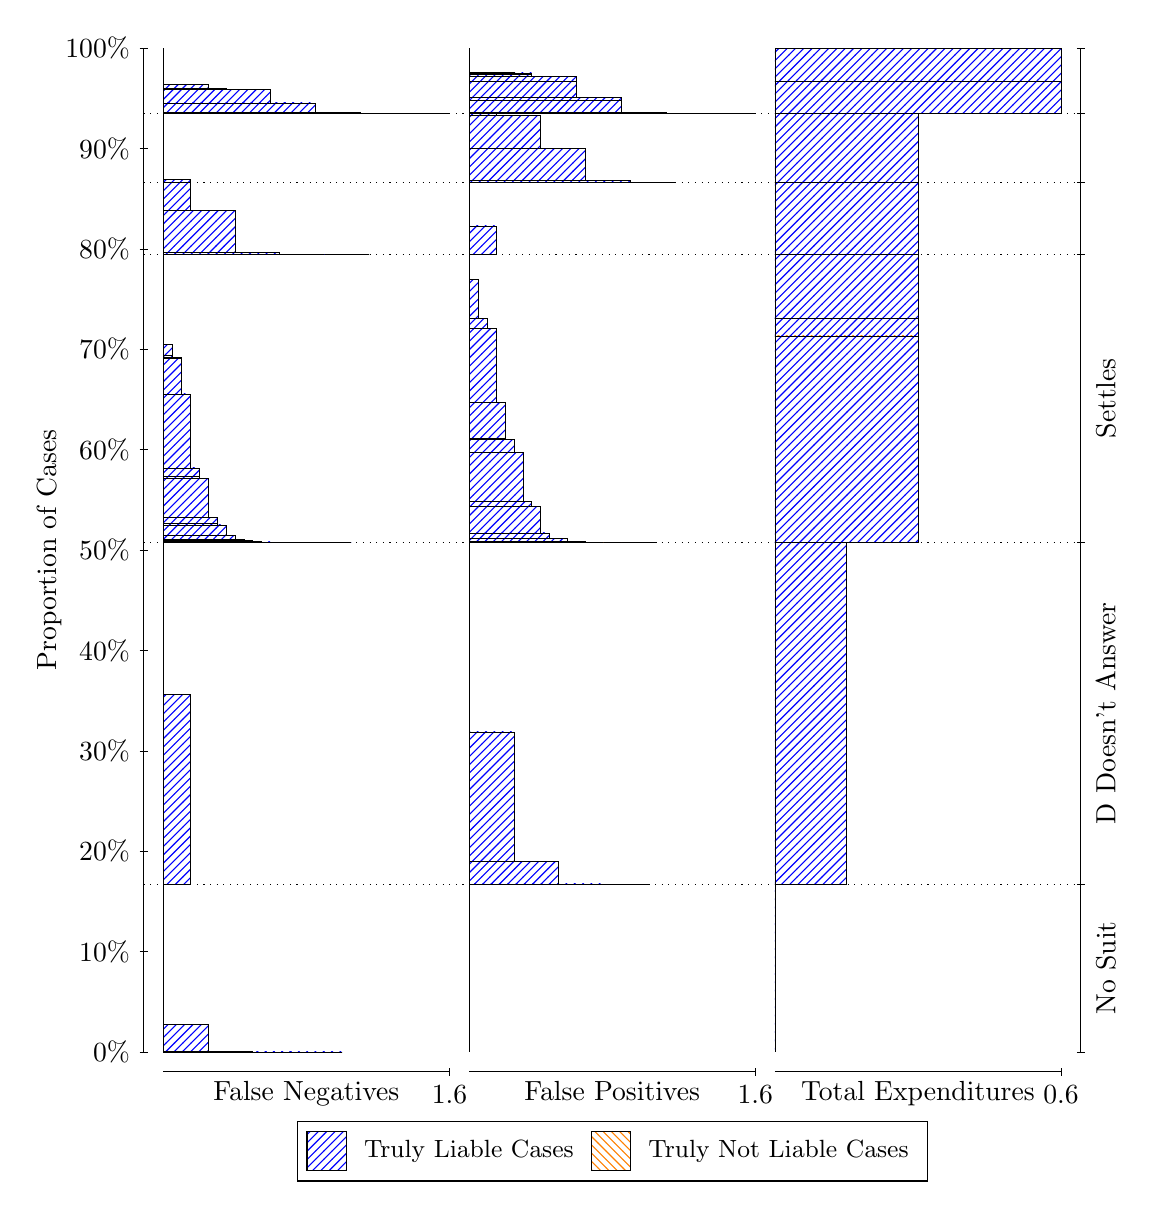
\begin{tikzpicture}
\draw[black, very thin] (1.5,1.75) -- (1.5,14.5);
\node[rotate=90, anchor=center] at (0.3, 8.125) {Proportion of Cases};
\draw[black, very thin] (1.45,1.75) -- (1.55,1.75);
\node[anchor=east] at (1.45, 1.75) {0\%};
\draw[black, very thin] (1.45,3.025) -- (1.55,3.025);
\node[anchor=east] at (1.45, 3.025) {10\%};
\draw[black, very thin] (1.45,4.3) -- (1.55,4.3);
\node[anchor=east] at (1.45, 4.3) {20\%};
\draw[black, very thin] (1.45,5.575) -- (1.55,5.575);
\node[anchor=east] at (1.45, 5.575) {30\%};
\draw[black, very thin] (1.45,6.85) -- (1.55,6.85);
\node[anchor=east] at (1.45, 6.85) {40\%};
\draw[black, very thin] (1.45,8.125) -- (1.55,8.125);
\node[anchor=east] at (1.45, 8.125) {50\%};
\draw[black, very thin] (1.45,9.4) -- (1.55,9.4);
\node[anchor=east] at (1.45, 9.4) {60\%};
\draw[black, very thin] (1.45,10.675) -- (1.55,10.675);
\node[anchor=east] at (1.45, 10.675) {70\%};
\draw[black, very thin] (1.45,11.95) -- (1.55,11.95);
\node[anchor=east] at (1.45, 11.95) {80\%};
\draw[black, very thin] (1.45,13.225) -- (1.55,13.225);
\node[anchor=east] at (1.45, 13.225) {90\%};
\draw[black, very thin] (1.45,14.5) -- (1.55,14.5);
\node[anchor=east] at (1.45, 14.5) {100\%};

\draw[black, very thin] (13.4,1.75) -- (13.4,14.5);
\draw[black, very thin] (13.35,1.75) -- (13.45,1.75);
\node[anchor=west] at (13.35, 1.75) {};
\draw[black, very thin] (13.35,3.8823) -- (13.45,3.8823);
\node[anchor=west] at (13.35, 3.8823) {};
\draw[black, very thin] (13.35,8.2245) -- (13.45,8.2245);
\node[anchor=west] at (13.35, 8.2245) {};
\draw[black, very thin] (13.35,11.879) -- (13.45,11.879);
\node[anchor=west] at (13.35, 11.879) {};
\draw[black, very thin] (13.35,12.795) -- (13.45,12.795);
\node[anchor=west] at (13.35, 12.795) {};
\draw[black, very thin] (13.35,13.672) -- (13.45,13.672);
\node[anchor=west] at (13.35, 13.672) {};
\draw[black, very thin] (13.35,14.5) -- (13.45,14.5);
\node[anchor=west] at (13.35, 14.5) {};

\draw[black, very thin, pattern color=blue, pattern=north east lines] (1.75,1.75) rectangle (4.0208,1.75);
\draw[black, very thin, pattern color=blue, pattern=north east lines] (1.75,1.75) rectangle (3.4531,1.75);
\draw[black, very thin, pattern color=blue, pattern=north east lines] (1.75,1.75) rectangle (2.8854,1.753);
\draw[black, very thin, pattern color=blue, pattern=north east lines] (1.75,1.753) rectangle (2.3177,2.0991);
\draw[black, very thin, pattern color=orange, pattern=north west lines] (1.75,2.0991) rectangle (1.75,2.0991);
\draw[black, very thin, pattern color=blue, pattern=north east lines] (1.75,2.0991) rectangle (1.75,3.8823);
\draw[black, very thin, pattern color=blue, pattern=north east lines] (1.75,3.8823) rectangle (2.0906,6.2908);
\draw[black, very thin, pattern color=orange, pattern=north west lines] (1.75,6.2908) rectangle (1.75,6.2908);
\draw[black, very thin, pattern color=blue, pattern=north east lines] (1.75,6.2908) rectangle (1.75,8.2245);
\draw[black, very thin, pattern color=blue, pattern=north east lines] (1.75,8.2245) rectangle (4.1344,8.2245);
\draw[black, very thin, pattern color=blue, pattern=north east lines] (1.75,8.2245) rectangle (3.9073,8.2245);
\draw[black, very thin, pattern color=blue, pattern=north east lines] (1.75,8.2245) rectangle (3.6802,8.2245);
\draw[black, very thin, pattern color=blue, pattern=north east lines] (1.75,8.2245) rectangle (3.5667,8.2245);
\draw[black, very thin, pattern color=blue, pattern=north east lines] (1.75,8.2245) rectangle (3.4531,8.2245);
\draw[black, very thin, pattern color=blue, pattern=north east lines] (1.75,8.2245) rectangle (3.3396,8.2245);
\draw[black, very thin, pattern color=blue, pattern=north east lines] (1.75,8.2245) rectangle (3.226,8.2245);
\draw[black, very thin, pattern color=blue, pattern=north east lines] (1.75,8.2245) rectangle (3.1125,8.2287);
\draw[black, very thin, pattern color=blue, pattern=north east lines] (1.75,8.2287) rectangle (2.999,8.231);
\draw[black, very thin, pattern color=blue, pattern=north east lines] (1.75,8.231) rectangle (2.8854,8.2473);
\draw[black, very thin, pattern color=blue, pattern=north east lines] (1.75,8.2473) rectangle (2.7719,8.2475);
\draw[black, very thin, pattern color=blue, pattern=north east lines] (1.75,8.2475) rectangle (2.7719,8.2576);
\draw[black, very thin, pattern color=blue, pattern=north east lines] (1.75,8.2576) rectangle (2.6583,8.3088);
\draw[black, very thin, pattern color=blue, pattern=north east lines] (1.75,8.3088) rectangle (2.5448,8.4449);
\draw[black, very thin, pattern color=blue, pattern=north east lines] (1.75,8.4449) rectangle (2.4312,8.4617);
\draw[black, very thin, pattern color=blue, pattern=north east lines] (1.75,8.4617) rectangle (2.4312,8.5432);
\draw[black, very thin, pattern color=blue, pattern=north east lines] (1.75,8.5432) rectangle (2.3177,9.0328);
\draw[black, very thin, pattern color=blue, pattern=north east lines] (1.75,9.0328) rectangle (2.2042,9.0626);
\draw[black, very thin, pattern color=blue, pattern=north east lines] (1.75,9.0626) rectangle (2.2042,9.1677);
\draw[black, very thin, pattern color=blue, pattern=north east lines] (1.75,9.1677) rectangle (2.0906,10.108);
\draw[black, very thin, pattern color=blue, pattern=north east lines] (1.75,10.108) rectangle (1.9771,10.565);
\draw[black, very thin, pattern color=blue, pattern=north east lines] (1.75,10.565) rectangle (1.9771,10.574);
\draw[black, very thin, pattern color=blue, pattern=north east lines] (1.75,10.574) rectangle (1.8635,10.595);
\draw[black, very thin, pattern color=blue, pattern=north east lines] (1.75,10.595) rectangle (1.8635,10.734);
\draw[black, very thin, pattern color=blue, pattern=north east lines] (1.75,10.734) rectangle (1.75,10.734);
\draw[black, very thin, pattern color=orange, pattern=north west lines] (1.75,10.734) rectangle (1.75,10.734);
\draw[black, very thin, pattern color=blue, pattern=north east lines] (1.75,10.734) rectangle (1.75,11.879);
\draw[black, very thin, pattern color=blue, pattern=north east lines] (1.75,11.879) rectangle (4.3615,11.879);
\draw[black, very thin, pattern color=blue, pattern=north east lines] (1.75,11.879) rectangle (3.7937,11.879);
\draw[black, very thin, pattern color=blue, pattern=north east lines] (1.75,11.879) rectangle (3.226,11.907);
\draw[black, very thin, pattern color=blue, pattern=north east lines] (1.75,11.907) rectangle (2.6583,12.434);
\draw[black, very thin, pattern color=blue, pattern=north east lines] (1.75,12.434) rectangle (2.0906,12.795);
\draw[black, very thin, pattern color=orange, pattern=north west lines] (1.75,12.795) rectangle (1.75,12.795);
\draw[black, very thin, pattern color=blue, pattern=north east lines] (1.75,12.795) rectangle (2.0906,12.827);
\draw[black, very thin, pattern color=orange, pattern=north west lines] (1.75,12.827) rectangle (1.75,12.827);
\draw[black, very thin, pattern color=blue, pattern=north east lines] (1.75,12.827) rectangle (1.75,13.672);
\draw[black, very thin, pattern color=blue, pattern=north east lines] (1.75,13.672) rectangle (5.3833,13.672);
\draw[black, very thin, pattern color=blue, pattern=north east lines] (1.75,13.672) rectangle (4.8156,13.672);
\draw[black, very thin, pattern color=blue, pattern=north east lines] (1.75,13.672) rectangle (4.2479,13.681);
\draw[black, very thin, pattern color=blue, pattern=north east lines] (1.75,13.681) rectangle (3.6802,13.802);
\draw[black, very thin, pattern color=blue, pattern=north east lines] (1.75,13.802) rectangle (3.4531,13.802);
\draw[black, very thin, pattern color=blue, pattern=north east lines] (1.75,13.802) rectangle (3.1125,13.977);
\draw[black, very thin, pattern color=blue, pattern=north east lines] (1.75,13.977) rectangle (2.8854,13.979);
\draw[black, very thin, pattern color=blue, pattern=north east lines] (1.75,13.979) rectangle (2.5448,13.988);
\draw[black, very thin, pattern color=blue, pattern=north east lines] (1.75,13.988) rectangle (2.3177,14.034);
\draw[black, very thin, pattern color=blue, pattern=north east lines] (1.75,14.034) rectangle (1.9771,14.034);
\draw[black, very thin, pattern color=orange, pattern=north west lines] (1.75,14.034) rectangle (1.75,14.034);
\draw[black, very thin, pattern color=blue, pattern=north east lines] (1.75,14.034) rectangle (1.75,14.5);
\draw[black, very thin, pattern color=orange, pattern=north west lines] (5.6333,1.75) rectangle (5.6333,1.75);
\draw[black, very thin, pattern color=blue, pattern=north east lines] (5.6333,1.75) rectangle (5.6333,3.8823);
\draw[black, very thin, pattern color=orange, pattern=north west lines] (5.6333,3.8823) rectangle (7.9042,3.8823);
\draw[black, very thin, pattern color=blue, pattern=north east lines] (5.6333,3.8823) rectangle (7.9042,3.8823);
\draw[black, very thin, pattern color=blue, pattern=north east lines] (5.6333,3.8823) rectangle (7.3365,3.8844);
\draw[black, very thin, pattern color=blue, pattern=north east lines] (5.6333,3.8844) rectangle (6.7687,4.1731);
\draw[black, very thin, pattern color=blue, pattern=north east lines] (5.6333,4.1731) rectangle (6.201,5.8159);
\draw[black, very thin, pattern color=blue, pattern=north east lines] (5.6333,5.8159) rectangle (5.6333,8.2245);
\draw[black, very thin, pattern color=orange, pattern=north west lines] (5.6333,8.2245) rectangle (8.0177,8.2245);
\draw[black, very thin, pattern color=blue, pattern=north east lines] (5.6333,8.2245) rectangle (8.0177,8.2245);
\draw[black, very thin, pattern color=orange, pattern=north west lines] (5.6333,8.2245) rectangle (7.7906,8.2245);
\draw[black, very thin, pattern color=blue, pattern=north east lines] (5.6333,8.2245) rectangle (7.7906,8.2245);
\draw[black, very thin, pattern color=orange, pattern=north west lines] (5.6333,8.2245) rectangle (7.5635,8.2245);
\draw[black, very thin, pattern color=blue, pattern=north east lines] (5.6333,8.2245) rectangle (7.5635,8.2245);
\draw[black, very thin, pattern color=blue, pattern=north east lines] (5.6333,8.2245) rectangle (7.45,8.2245);
\draw[black, very thin, pattern color=orange, pattern=north west lines] (5.6333,8.2245) rectangle (7.3365,8.2245);
\draw[black, very thin, pattern color=blue, pattern=north east lines] (5.6333,8.2245) rectangle (7.3365,8.2245);
\draw[black, very thin, pattern color=blue, pattern=north east lines] (5.6333,8.2245) rectangle (7.2229,8.2245);
\draw[black, very thin, pattern color=orange, pattern=north west lines] (5.6333,8.2245) rectangle (7.1094,8.2245);
\draw[black, very thin, pattern color=blue, pattern=north east lines] (5.6333,8.2245) rectangle (7.1094,8.2385);
\draw[black, very thin, pattern color=blue, pattern=north east lines] (5.6333,8.2385) rectangle (6.9958,8.2387);
\draw[black, very thin, pattern color=orange, pattern=north west lines] (5.6333,8.2387) rectangle (6.8823,8.2387);
\draw[black, very thin, pattern color=blue, pattern=north east lines] (5.6333,8.2387) rectangle (6.8823,8.2739);
\draw[black, very thin, pattern color=orange, pattern=north west lines] (5.6333,8.2739) rectangle (6.8823,8.2739);
\draw[black, very thin, pattern color=blue, pattern=north east lines] (5.6333,8.2739) rectangle (6.8823,8.2739);
\draw[black, very thin, pattern color=blue, pattern=north east lines] (5.6333,8.2739) rectangle (6.7687,8.2741);
\draw[black, very thin, pattern color=blue, pattern=north east lines] (5.6333,8.2741) rectangle (6.6552,8.2754);
\draw[black, very thin, pattern color=orange, pattern=north west lines] (5.6333,8.2754) rectangle (6.6552,8.2754);
\draw[black, very thin, pattern color=blue, pattern=north east lines] (5.6333,8.2754) rectangle (6.6552,8.3437);
\draw[black, very thin, pattern color=blue, pattern=north east lines] (5.6333,8.3437) rectangle (6.5417,8.6778);
\draw[black, very thin, pattern color=orange, pattern=north west lines] (5.6333,8.6778) rectangle (6.4281,8.6778);
\draw[black, very thin, pattern color=blue, pattern=north east lines] (5.6333,8.6778) rectangle (6.4281,8.7397);
\draw[black, very thin, pattern color=blue, pattern=north east lines] (5.6333,8.7397) rectangle (6.3146,9.3695);
\draw[black, very thin, pattern color=blue, pattern=north east lines] (5.6333,9.3695) rectangle (6.3146,9.3696);
\draw[black, very thin, pattern color=orange, pattern=north west lines] (5.6333,9.3696) rectangle (6.201,9.3696);
\draw[black, very thin, pattern color=blue, pattern=north east lines] (5.6333,9.3696) rectangle (6.201,9.5295);
\draw[black, very thin, pattern color=blue, pattern=north east lines] (5.6333,9.5295) rectangle (6.0875,9.5381);
\draw[black, very thin, pattern color=blue, pattern=north east lines] (5.6333,9.5381) rectangle (6.0875,9.9954);
\draw[black, very thin, pattern color=blue, pattern=north east lines] (5.6333,9.9954) rectangle (5.974,10.935);
\draw[black, very thin, pattern color=blue, pattern=north east lines] (5.6333,10.935) rectangle (5.8604,11.07);
\draw[black, very thin, pattern color=blue, pattern=north east lines] (5.6333,11.07) rectangle (5.7469,11.559);
\draw[black, very thin, pattern color=blue, pattern=north east lines] (5.6333,11.559) rectangle (5.7469,11.56);
\draw[black, very thin, pattern color=blue, pattern=north east lines] (5.6333,11.56) rectangle (5.6333,11.879);
\draw[black, very thin, pattern color=orange, pattern=north west lines] (5.6333,11.879) rectangle (5.974,11.879);
\draw[black, very thin, pattern color=blue, pattern=north east lines] (5.6333,11.879) rectangle (5.974,12.24);
\draw[black, very thin, pattern color=blue, pattern=north east lines] (5.6333,12.24) rectangle (5.6333,12.795);
\draw[black, very thin, pattern color=orange, pattern=north west lines] (5.6333,12.795) rectangle (8.2448,12.795);
\draw[black, very thin, pattern color=blue, pattern=north east lines] (5.6333,12.795) rectangle (8.2448,12.795);
\draw[black, very thin, pattern color=blue, pattern=north east lines] (5.6333,12.795) rectangle (7.6771,12.816);
\draw[black, very thin, pattern color=blue, pattern=north east lines] (5.6333,12.816) rectangle (7.1094,13.228);
\draw[black, very thin, pattern color=blue, pattern=north east lines] (5.6333,13.228) rectangle (6.5417,13.64);
\draw[black, very thin, pattern color=blue, pattern=north east lines] (5.6333,13.64) rectangle (5.974,13.672);
\draw[black, very thin, pattern color=orange, pattern=north west lines] (5.6333,13.672) rectangle (9.2667,13.672);
\draw[black, very thin, pattern color=blue, pattern=north east lines] (5.6333,13.672) rectangle (9.2667,13.672);
\draw[black, very thin, pattern color=orange, pattern=north west lines] (5.6333,13.672) rectangle (8.699,13.672);
\draw[black, very thin, pattern color=blue, pattern=north east lines] (5.6333,13.672) rectangle (8.699,13.672);
\draw[black, very thin, pattern color=orange, pattern=north west lines] (5.6333,13.672) rectangle (8.1313,13.672);
\draw[black, very thin, pattern color=blue, pattern=north east lines] (5.6333,13.672) rectangle (8.1313,13.687);
\draw[black, very thin, pattern color=blue, pattern=north east lines] (5.6333,13.687) rectangle (7.5635,13.837);
\draw[black, very thin, pattern color=orange, pattern=north west lines] (5.6333,13.837) rectangle (7.5635,13.837);
\draw[black, very thin, pattern color=blue, pattern=north east lines] (5.6333,13.837) rectangle (7.5635,13.87);
\draw[black, very thin, pattern color=blue, pattern=north east lines] (5.6333,13.87) rectangle (6.9958,14.076);
\draw[black, very thin, pattern color=blue, pattern=north east lines] (5.6333,14.076) rectangle (6.9958,14.138);
\draw[black, very thin, pattern color=orange, pattern=north west lines] (5.6333,14.138) rectangle (6.7687,14.138);
\draw[black, very thin, pattern color=blue, pattern=north east lines] (5.6333,14.138) rectangle (6.7687,14.138);
\draw[black, very thin, pattern color=blue, pattern=north east lines] (5.6333,14.138) rectangle (6.4281,14.17);
\draw[black, very thin, pattern color=blue, pattern=north east lines] (5.6333,14.17) rectangle (6.4281,14.184);
\draw[black, very thin, pattern color=orange, pattern=north west lines] (5.6333,14.184) rectangle (6.201,14.184);
\draw[black, very thin, pattern color=blue, pattern=north east lines] (5.6333,14.184) rectangle (6.201,14.193);
\draw[black, very thin, pattern color=blue, pattern=north east lines] (5.6333,14.193) rectangle (5.8604,14.194);
\draw[black, very thin, pattern color=blue, pattern=north east lines] (5.6333,14.194) rectangle (5.8604,14.195);
\draw[black, very thin, pattern color=orange, pattern=north west lines] (5.6333,14.195) rectangle (5.6333,14.195);
\draw[black, very thin, pattern color=blue, pattern=north east lines] (5.6333,14.195) rectangle (5.6333,14.5);
\draw[black, very thin, pattern color=orange, pattern=north west lines] (9.5167,1.75) rectangle (9.5167,1.75);
\draw[black, very thin, pattern color=blue, pattern=north east lines] (9.5167,1.75) rectangle (9.5167,3.8823);
\draw[black, very thin, pattern color=orange, pattern=north west lines] (9.5167,3.8823) rectangle (10.425,3.8823);
\draw[black, very thin, pattern color=blue, pattern=north east lines] (9.5167,3.8823) rectangle (10.425,8.2245);
\draw[black, very thin, pattern color=orange, pattern=north west lines] (9.5167,8.2245) rectangle (11.333,8.2245);
\draw[black, very thin, pattern color=blue, pattern=north east lines] (9.5167,8.2245) rectangle (11.333,10.844);
\draw[black, very thin, pattern color=orange, pattern=north west lines] (9.5167,10.844) rectangle (11.333,10.844);
\draw[black, very thin, pattern color=blue, pattern=north east lines] (9.5167,10.844) rectangle (11.333,11.066);
\draw[black, very thin, pattern color=orange, pattern=north west lines] (9.5167,11.066) rectangle (11.333,11.066);
\draw[black, very thin, pattern color=blue, pattern=north east lines] (9.5167,11.066) rectangle (11.333,11.879);
\draw[black, very thin, pattern color=orange, pattern=north west lines] (9.5167,11.879) rectangle (11.333,11.879);
\draw[black, very thin, pattern color=blue, pattern=north east lines] (9.5167,11.879) rectangle (11.333,12.795);
\draw[black, very thin, pattern color=orange, pattern=north west lines] (9.5167,12.795) rectangle (11.333,12.795);
\draw[black, very thin, pattern color=blue, pattern=north east lines] (9.5167,12.795) rectangle (11.333,13.672);
\draw[black, very thin, pattern color=orange, pattern=north west lines] (9.5167,13.672) rectangle (13.15,13.672);
\draw[black, very thin, pattern color=blue, pattern=north east lines] (9.5167,13.672) rectangle (13.15,14.074);
\draw[black, very thin, pattern color=orange, pattern=north west lines] (9.5167,14.074) rectangle (13.15,14.074);
\draw[black, very thin, pattern color=blue, pattern=north east lines] (9.5167,14.074) rectangle (13.15,14.5);
\draw[black, dotted] (1.5,3.8823) -- (13.4,3.8823);
\draw[black, dotted] (1.5,8.2245) -- (13.4,8.2245);
\draw[black, dotted] (1.5,11.879) -- (13.4,11.879);
\draw[black, dotted] (1.5,12.795) -- (13.4,12.795);
\draw[black, dotted] (1.5,13.672) -- (13.4,13.672);
\draw[black, very thin] (1.75,1.5) -- (5.3833,1.5);
\node[anchor=north] at (3.5667, 1.5) {False Negatives};
\draw[black, very thin] (5.3833,1.45) -- (5.3833,1.55);
\node[anchor=north] at (5.3833, 1.45) {1.6};

\draw[black, very thin] (5.6333,1.5) -- (9.2667,1.5);
\node[anchor=north] at (7.45, 1.5) {False Positives};
\draw[black, very thin] (9.2667,1.45) -- (9.2667,1.55);
\node[anchor=north] at (9.2667, 1.45) {1.6};

\draw[black, very thin] (9.5167,1.5) -- (13.15,1.5);
\node[anchor=north] at (11.333, 1.5) {Total Expenditures};
\draw[black, very thin] (13.15,1.45) -- (13.15,1.55);
\node[anchor=north] at (13.15, 1.45) {0.6};

\node[black, centered, rotate=90] at (13.72, 2.8162) {No Suit};
\node[black, centered, rotate=90] at (13.72, 6.0534) {D Doesn't Answer};
\node[black, centered, rotate=90] at (13.72, 10.052) {Settles};




\draw (7.449999999999999,1.5) node[draw=none] (baseCoordinate) {};
\begin{scope}[align=center]
        \matrix[scale=0.5, draw=black, below=0.5cm of baseCoordinate, nodes={draw}, column sep=0.1cm]{
            \node[rectangle, draw, minimum width=0.5cm, minimum height=0.5cm, pattern=north east lines, pattern color=blue] {}; &
            \node[draw=none, font=\small] (B) {Truly Liable Cases}; &
            \node[rectangle, draw, minimum width=0.5cm, minimum height=0.5cm, pattern=north west lines, pattern color=orange] {}; &
            \node[draw=none, font=\small] (B) {Truly Not Liable Cases}; \\
            };
\end{scope}

\end{tikzpicture}
\end{document}